\chapter{Solution validation}

\section {Data model}

The model designed for the Observatory project represented in figure~\ref{fig:datamodel-obsproject} is a simplification of the ALMA Project Data Model summarized in section~\ref{sec:apdm} and it is the model used in the ALMA's Dynamic Scheduling Algorithm briefly described in section~\ref{sec:alma-dsa}.

The most relevant parts are: 
\begin{description}
\item[bla1] \hfill \\
Description of bla1
\end{description}

\begin{figure}[]	
\begin{center}
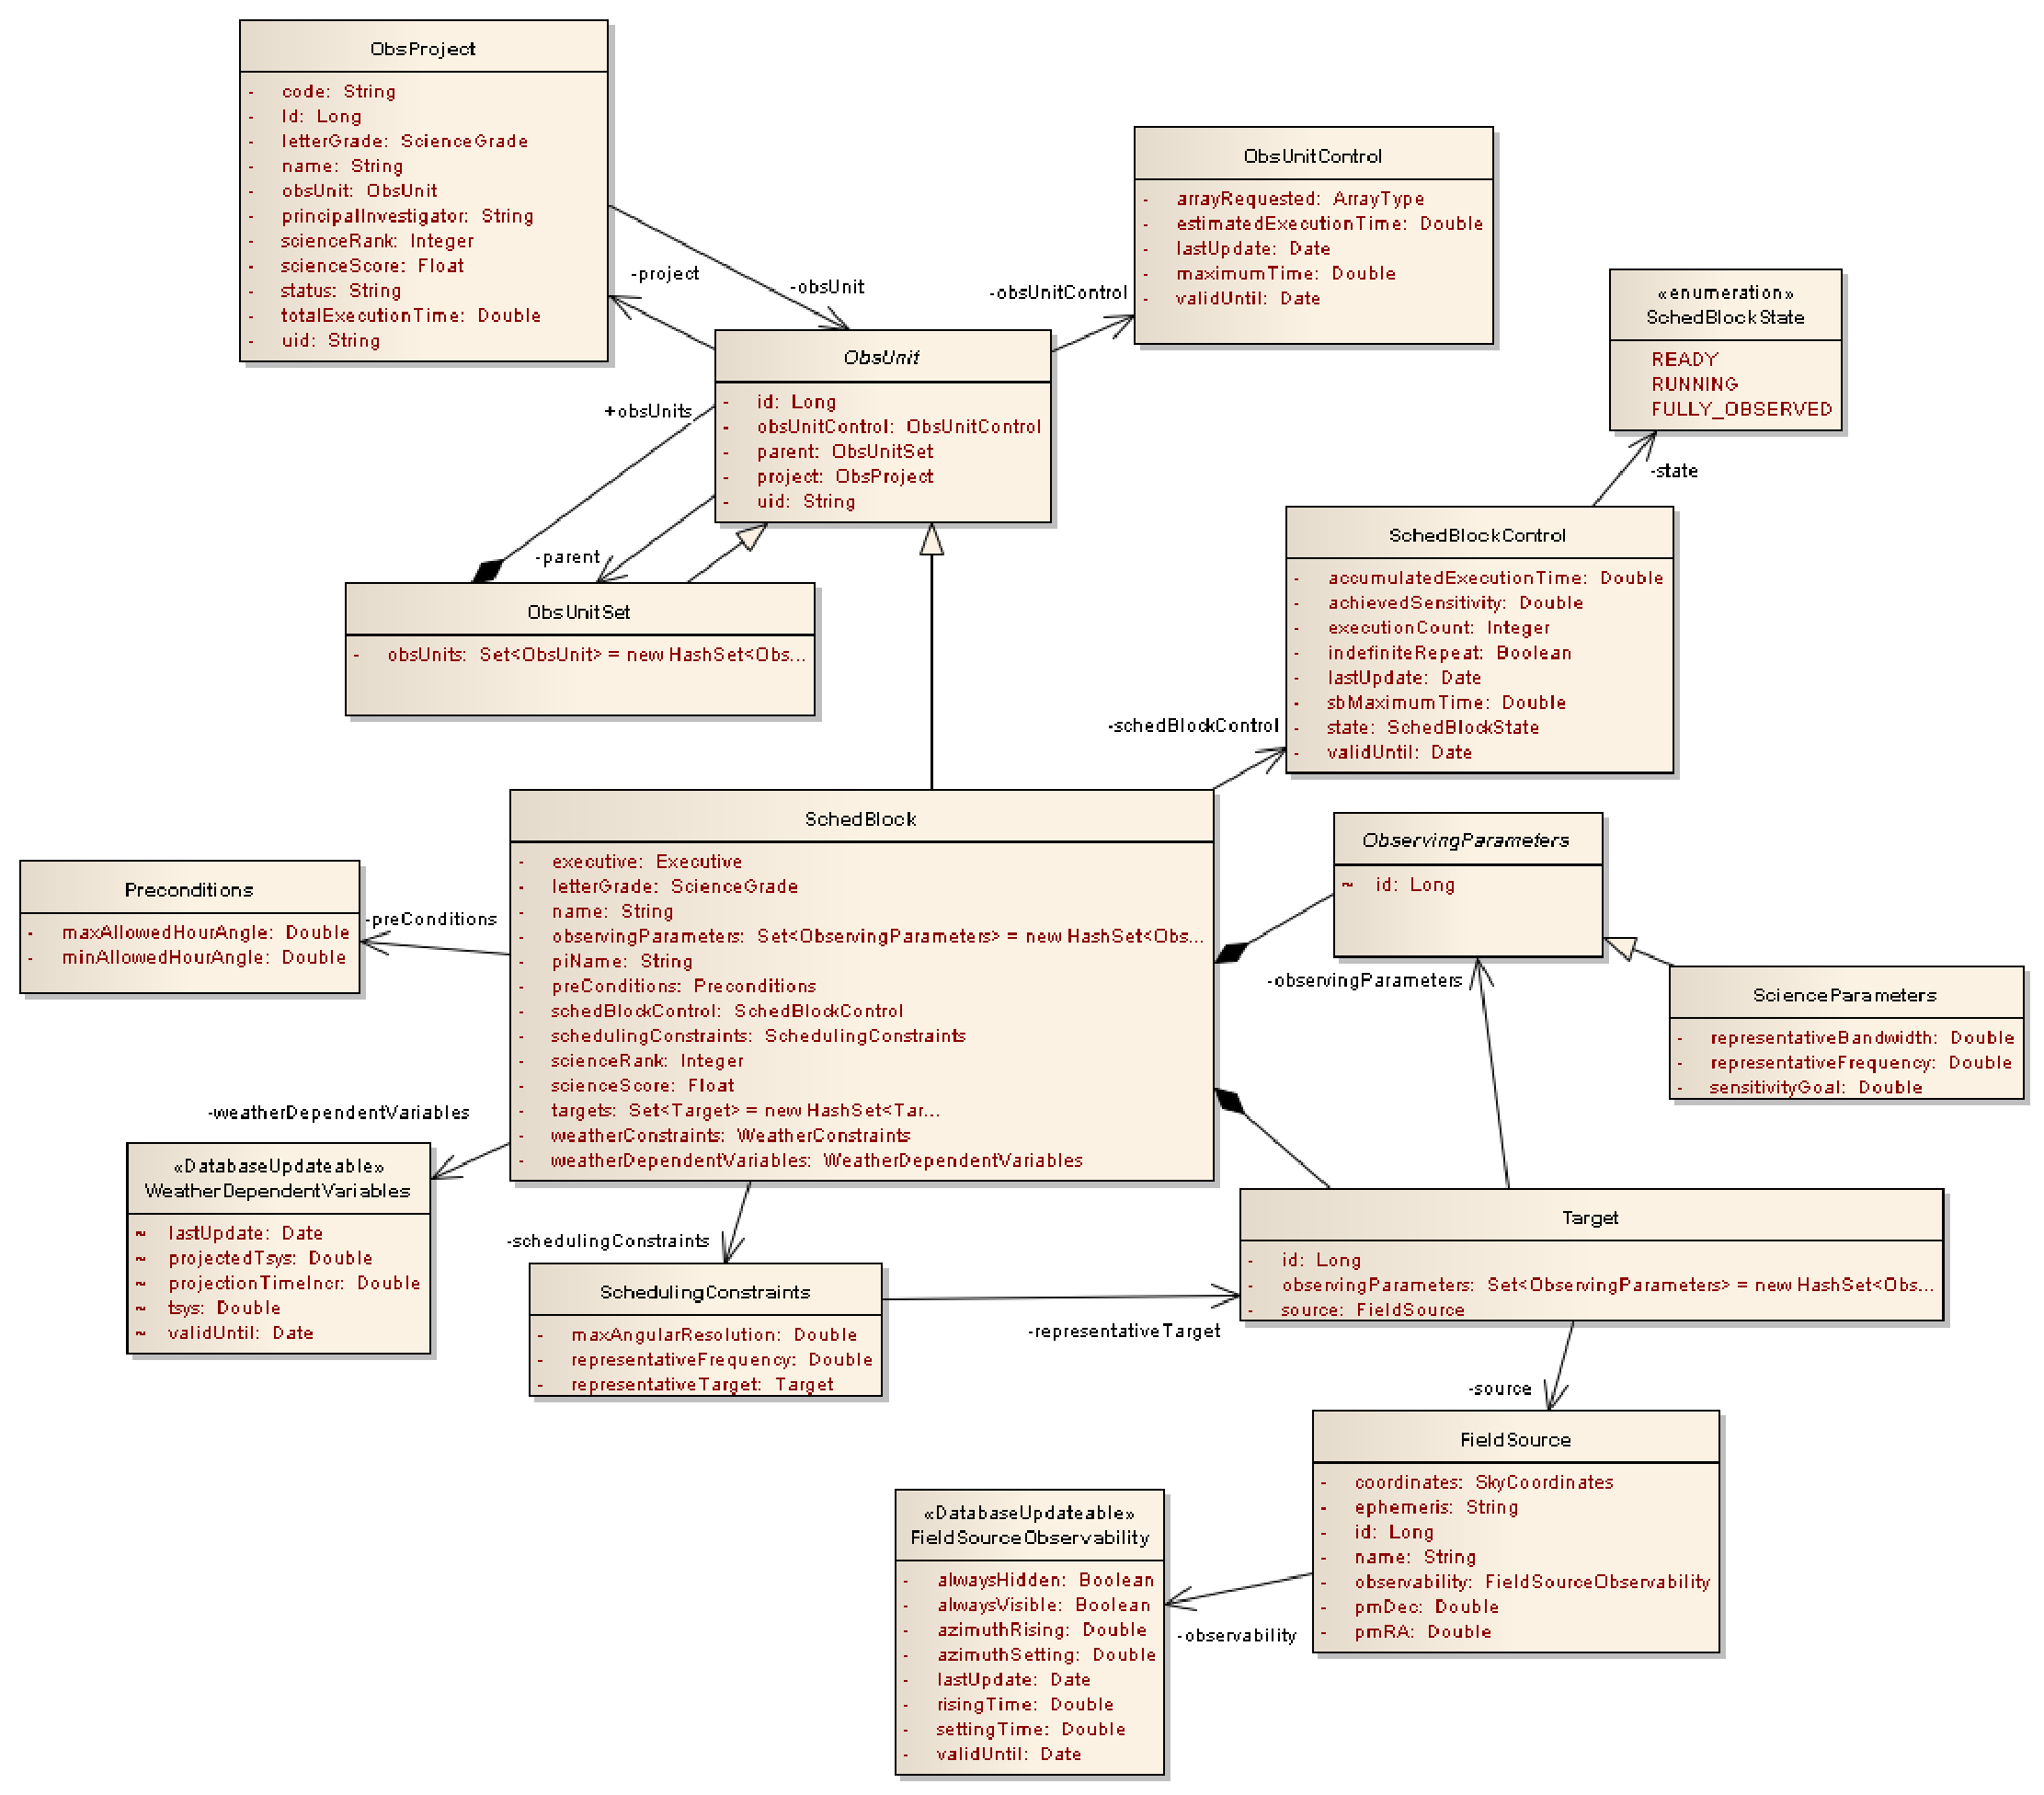
\includegraphics[width=1.15\textwidth]{images/ObsProject}
\caption{Observation Project data model}
\end{center}
\label{fig:datamodel-obsproject}
\end{figure}

The model designed for handle the observatory instrumentation is represented in figure~\ref{fig:datamodel-observatory}

\begin{figure}[]	
\begin{center}
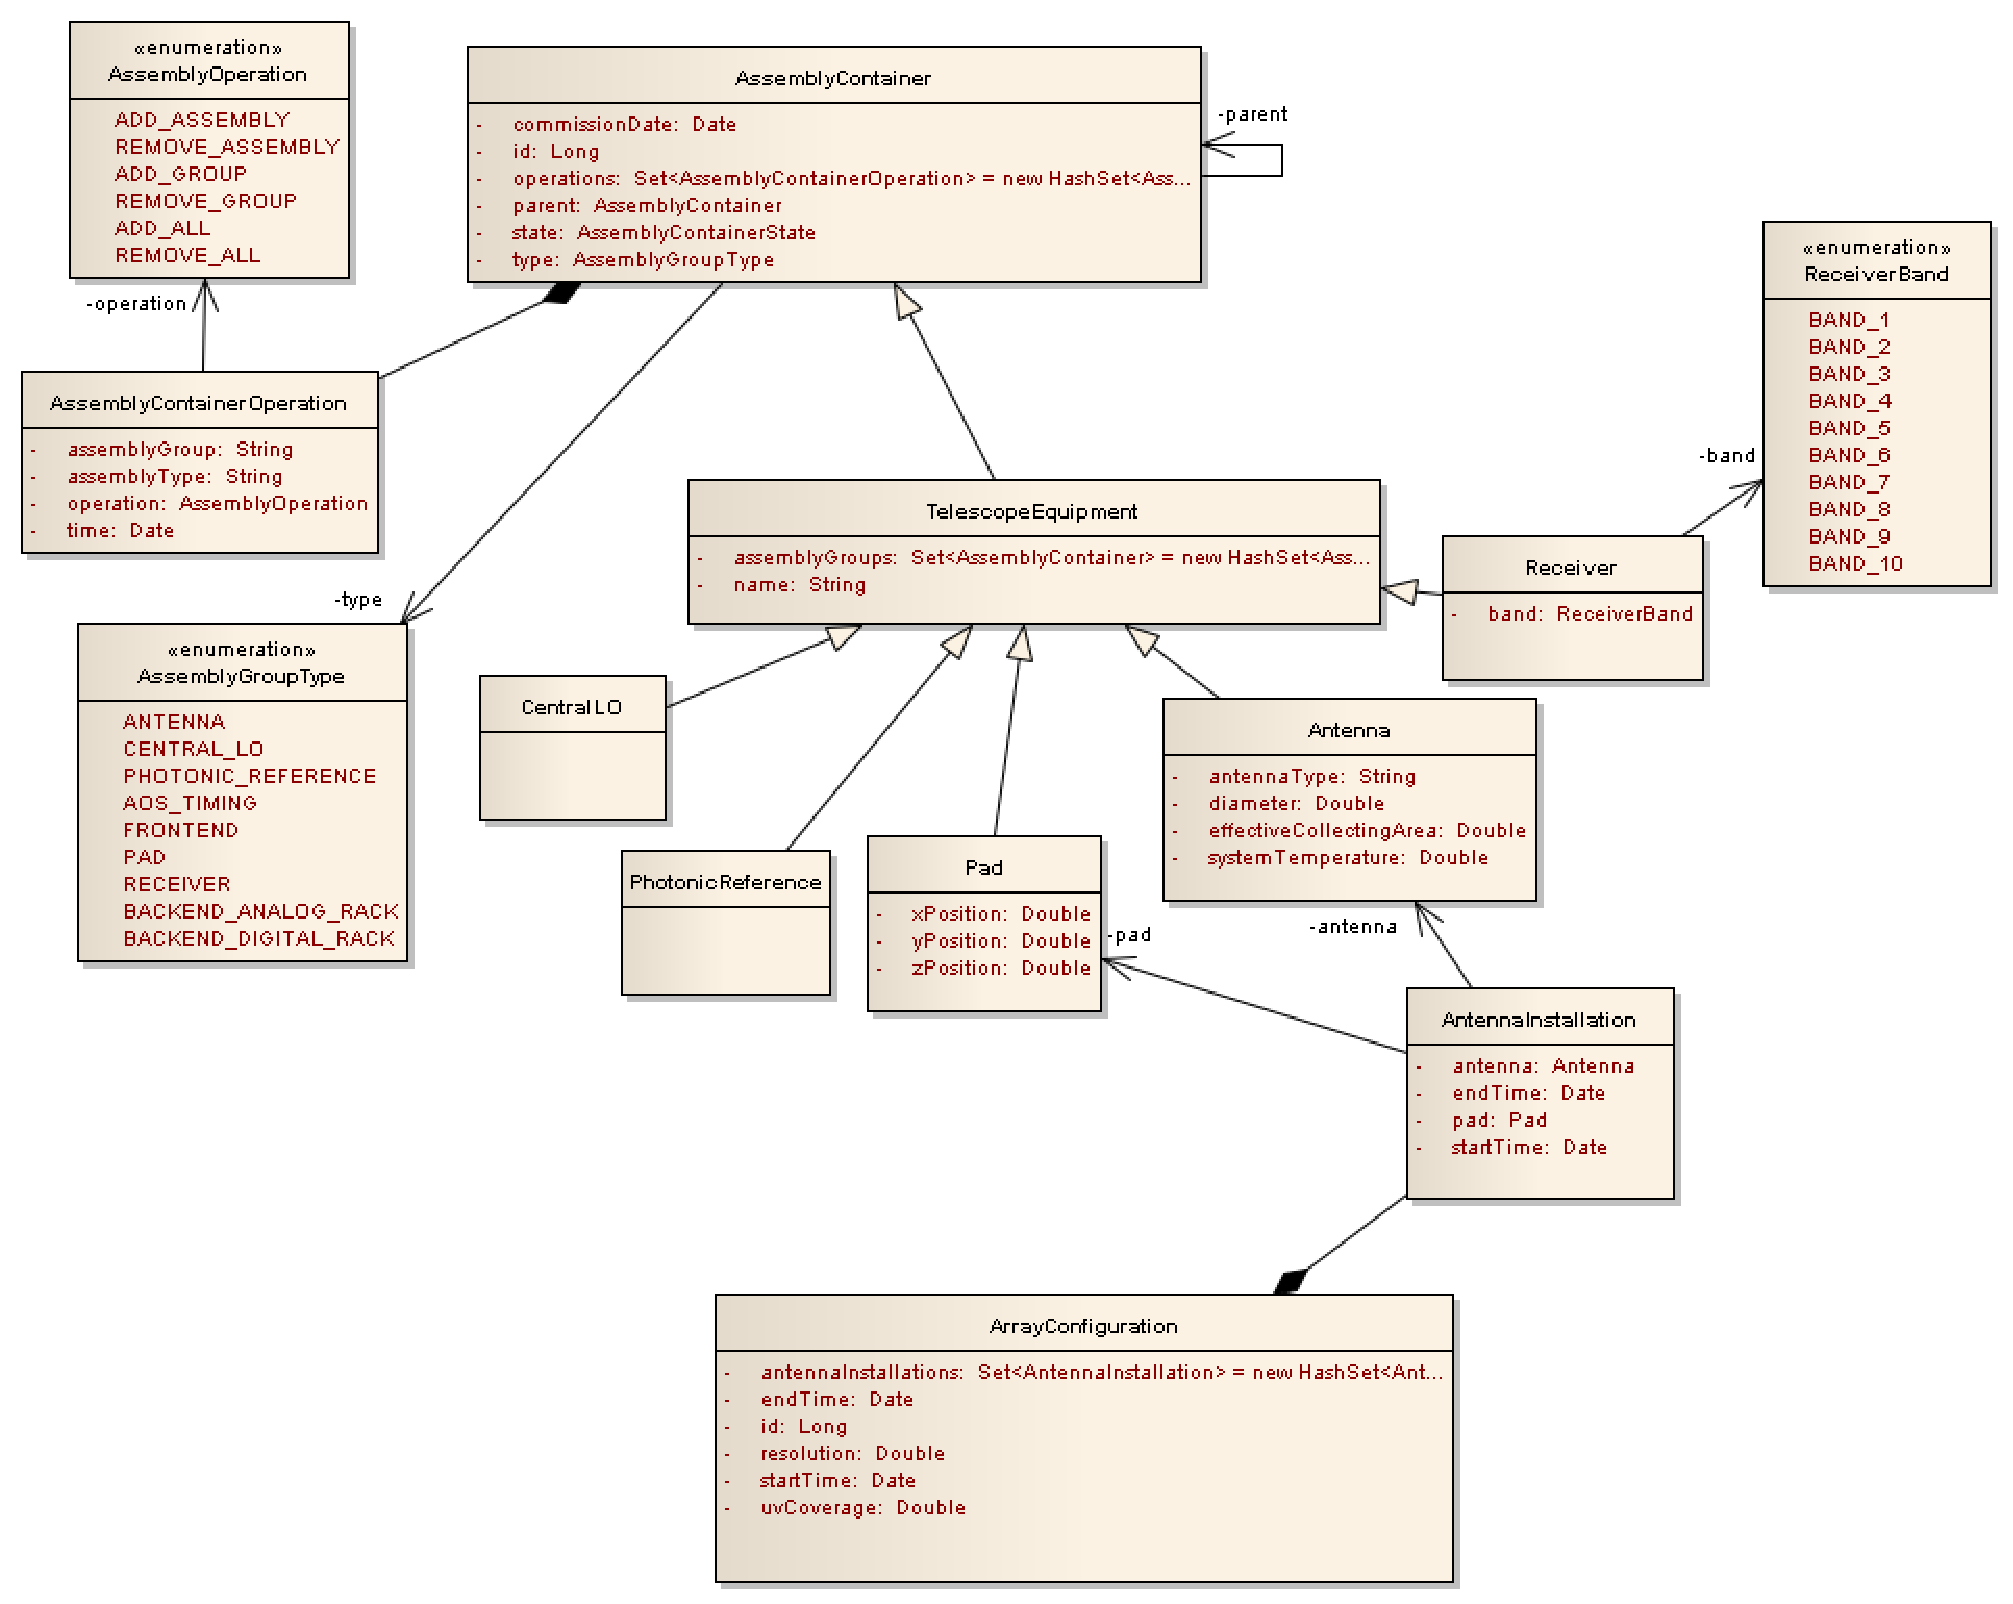
\includegraphics[width=\textwidth]{images/Observatory}
\caption{Observatory instrumentation data model}
\end{center}
\label{fig:datamodel-observatory}
\end{figure}

The model designed for handle the Executive information and the observing season is represented in figure~\ref{fig:datamodel-executive}

\begin{figure}[]	
\begin{center}
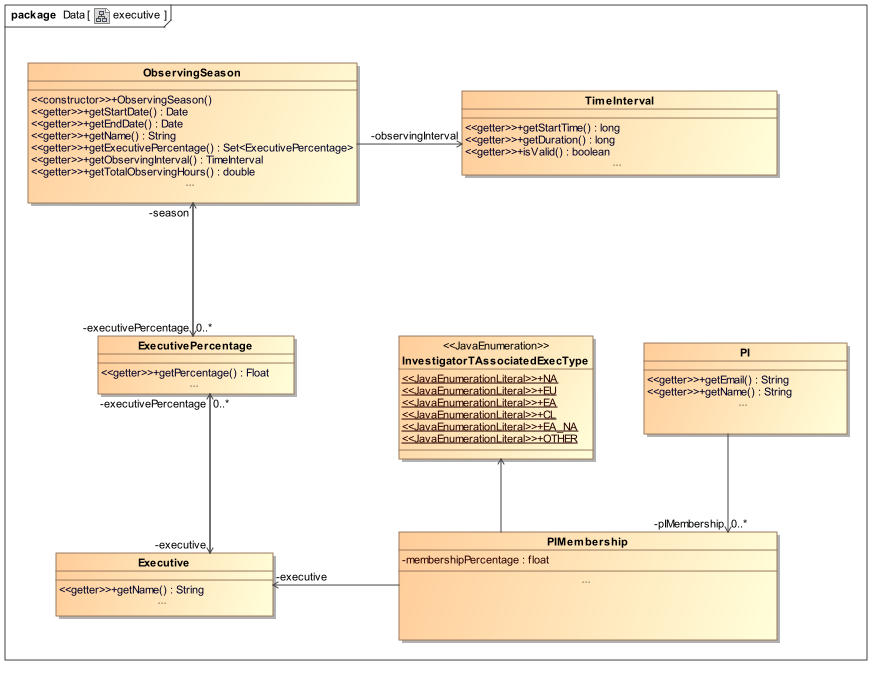
\includegraphics[width=\textwidth]{images/Executive}
\caption{Executive and observing season data model}
\end{center}
\label{fig:datamodel-executive}
\end{figure}

The model designed for handle the weather is represented in figure~\ref{fig:datamodel-weather}

\begin{figure}[]	
\begin{center}
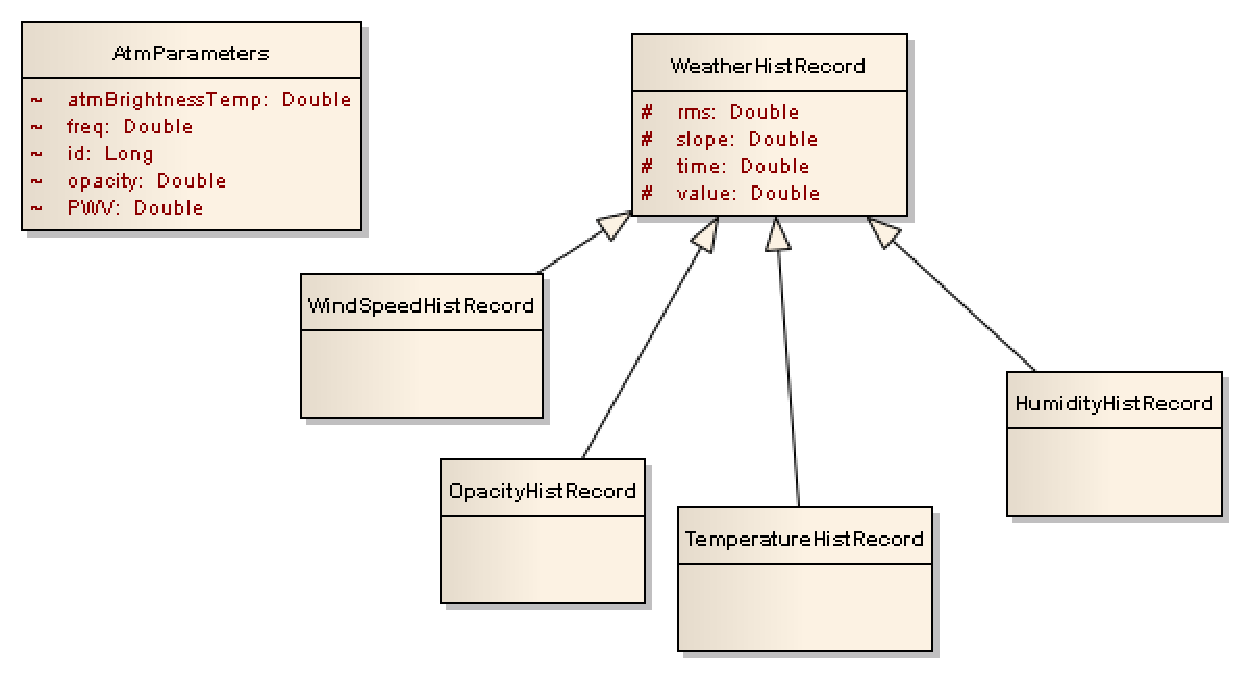
\includegraphics[width=\textwidth]{images/Weather}
\caption{Executive and observing season data model}
\end{center}
\label{fig:datamodel-weather}
\end{figure}

\section {Simulation}

\begin{figure}[]	
\begin{center}
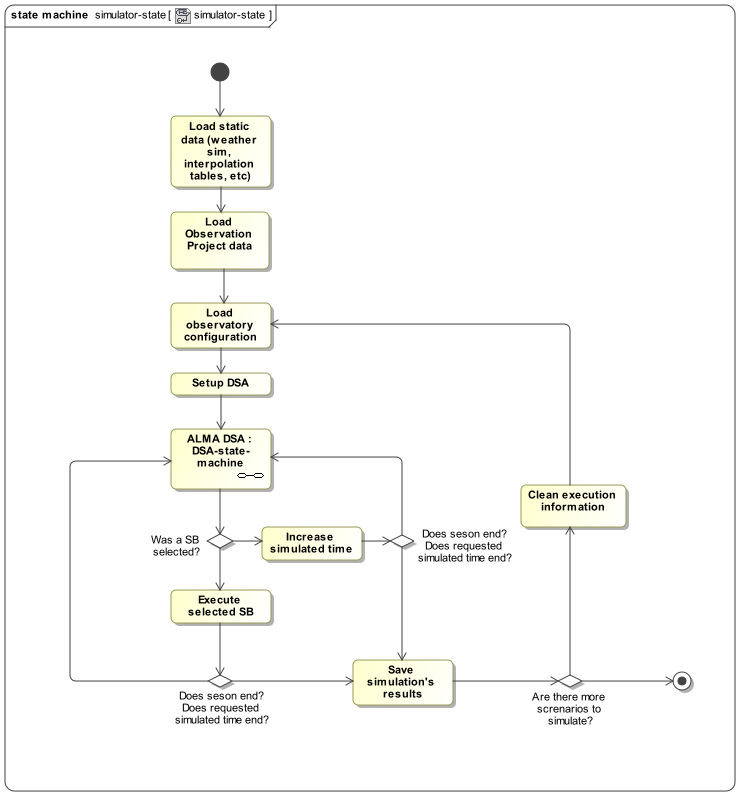
\includegraphics[width=\textwidth]{images/simulator-state-machine}
\caption{ALMA simulator's state machine}
\end{center}
\label{fig:sim-state-machine}
\end{figure}

\section {Algorithm implementation}

\section {Input Observation projects}